\documentclass[11pt,letterpaper,twocolumn]{article}
\setlength{\columnsep}{0.75cm}
\usepackage[utf8]{inputenc}
\usepackage{amsmath}
\usepackage{amsfonts}
\usepackage{amssymb}
\usepackage{graphicx}
\usepackage{wrapfig}
\author{Ben Shulman}
\begin{document}
\title{Vote Prediction in the House of Representatives}
\author{Benjamin Shulman, Jisha Kambo, John Oliver}
\date{December 13, 2012}
\maketitle

\section{Introduction}
The federal government of the United States is organized into three branches: Executive, Legislative and Judicial. The legislative branch (Congress) is responsible for sponsoring bills and voting on whether bills should become law. The United States Congress is divided into two sections, the House of Representatives and the Senate. The House of Representatives is made up of 435 representatives, each of which are elected every two years. The Senate is made up of 100 senators, 2 from each state and are elected on staggered six year cycles. The general process for a bill becoming a law is as follows. Each bill has a sponsor and is introduced to the House of Representatives, the bill then goes to committee and then is revised, researched and then sent to the House. The bill is debated by the representatives, and changes and amendments are recommended. The bill is then voted on by the members of the House. If it passes it is sent to the Senate where it goes through a similar process. If it is passed by the Senate it is sent to the president to be signed.

	A new law passed by Congress may have vast effects on American citizens and corporations, affecting revenue, assets, income, rights and freedoms. If citizens and corporations could know whether a bill would be passed by Congress before it was voted on it would give them advance warning such that they can lobby for changes to the bill, lobby for it to be shut down or passed or prepare themselves for the resulting effects. Further, if an individual representative or senator's vote could be predicted for a given bill it could give insights into the actual beliefs and platform of that congressperson. With these reasons in mind we will tackle the problem of vote prediction in the House of Representatives. We will approach the problem by treating each representative as a separate prediction problem and then use those predictions to predict whether  a bill will pass the House of Representatives. There has been very little exploration of this space, the only related work being done using the text bills to predict roll call votes by extending the ideal point model (Gerrish and Blei). Our work will focus not on the bill text, but on metadata about the bill and does not extend the ideal point model.

	In the following sections we will discuss our methodology for modeling and vote prediction. We examine and discuss our data extraction and feature selection. Further we show that bill metadata can be used to accurately predict the votes of individual representatives in the House using Support Vector Machines and compare our results against a baseline model for how representative's vote. 

\section{The Problem}
We are specifically interested in two questions: 
\begin{enumerate}
\item Can we predict an individual member of the House of Representative's vote on a bill with high accuracy in comparison to a baseline prediction model?
\item Can we use prediction of individual representative's vote to successfully predict whether a bill will be passed by the House of Representatives?
\end{enumerate}

\noindent Other questions we were interested in, but do not directly address in this publication are:

\begin{enumerate}
\item What features of a bill are most important to members of the House when voting?
\item What machine learning algorithms are most effective for this problem?
\end{enumerate}

\section{Algorithms and Methods}
To address our first question we focused primarily on using support vector machines to predict how each Representative would vote. For each representative we trained, tuned using a validation set and tested a separate support vector machine. To compare the success of support vector machines in predicting representatives' votes we used a baseline hypothesis which predicted that if a representative was of the same party as the sponsor of the bill he or she would vote "Yea" or if not, would vote "Nay." To predict whether a bill would be passed or not we did not use a standard machine learning algorithm as we had already done the prediction part using the individual support vector machines that predicted representatives' votes. Instead we used a simple algorithm that took a sum of predicted votes, where each vote is weighted by the accuracy of the representative's support vector machine on the test set for that representative. 

\section{Methodology}

\subsection{Data}

We took data from www.govtrack.us, a website promoting government transparency. From Govtrack's database we pulled data about all current representatives. We excluded five representatives from our experiment as there were problems with their information in the database, leaving us with 430 representatives. We used Govtrack's database to extract the voting records of these 430 representatives. For each representative we pulled all bills which were being voted on for passage which they had ever voted on. Each bill represented an example for a representative. The data from the database about each bill included information about the status of the bill; when it was introduced; congress number; when it was voted on; its title; and information about the sponsor of the bill such as name, district, and party. 

A month after we pulled all the bills which the current members of the House had voted on we pulled the six which had been voted on for passage in that month. These bills we then used to predict if the bill would pass or not.

\subsection{Feature Selection}
Feature set:
\begin{itemize}
\item Party of bill sponsor
\item Name of bill sponsor
\item District of bill sponsor
\item Gender of bill sponsor
\item Date bill sponsor joined House of Representatives
\item Whether bill sponsor has Twitter
\item Whether bill sponsor has a website
\item Whether sponsor has a nickname
\item Length of time bill has been alive
\item Congressional Session
\item Year the bill was introduced
\item Day the bill was voted on
\item Month the bill was voted on
\item Year the bill was voted on
\item Year the bill was voted on mod 2
\item Year the bill was voted on mod 4
\item Year the bill was voted on mod 6
\end{itemize}

	From the information we pulled from each bill we selected a set of features we wanted to consider in our models. The first was the party of the bill sponsor, we believe that representative's are likely to be have party bias and thus this is an important feature. We also used the sponsor's gender, as some representatives may have gender bias. Further we chose the sponsor's district and name as well, as representative's vote may be dependent upon certain districts or sponsors. For each representative, a bill sponsor's district and name were each a binary feature. Meaning if there were ten training bills for a representative, there may be up to ten features for sponsor name and up to ten for sponsor district. Final sponsor information we used as features were the date the sponsor joined the House, whether he or she had a Twitter, whether he or she had a website, and finally whether he or she had a nickname--each of these features were considered important as they could be indicators of the influence, popularity and experience of the sponsor which may be relevant to the voting representative.
	
	We included several other pieces of information about the bill. We extracted seven features from the date of the vote on the bill: the day of the vote, the month of the vote, the year of the vote, the year mod two, the year mod four and the year mod six. The day, month and year may all matter as priorities change given the time of year. The three modded year features align with voting cycles: representatives are elected every two years, president every four and senators every six. Thus if a representative was running in one of those elections, the time in relation to the cycle may affect his or her vote. Finally we included the congressional session in which the bill was voted on and the length of time the bill was active in days before it was voted on. These two features were included as the length of time a bill is debated for may effect votes as well as the session in which it is voted on. All of these features became the feature set we used in our models.

\subsection{Model Selection}

The machine learning model we chose to use for representative prediction tasks was a support vector machine. We treated each representative as a separate prediction task. Thus we had a separate data set for each member of the House. We split each data set into training, validation and testing sets. Thirty percent of the data for each member was used for testing, the remaining seventy percent was split between training and validation, with eighty percent going to training and twenty percent to validation. Then for each representative we trained, and tuned a separate support vector machine with a linear kernel, using the validation set to pick the best C value from five options $[0.0001, 0.001, 0.01, 0.05, 0.1]$. All support vector machine models were done in Python using the scikit-learn library. Thus we had 430 separate support vector machines. We tested each tuned support vector machine on the test set, recording the bills on which the support vector machine incorrectly predicted the House member's vote as well as the accuracy. We then tested our baseline model, which predicts that a representative will vote "yea" if he or she aligns with the same party as the bill sponsor and "nay" otherwise. 

To predict the outcome of a vote on bill passage we created a model which combined our individual predictions of representatives' votes into a single prediction. To do this we used a simple model which used predictions for a given bill to compute a weighted sum of votes. Each vote was weighted by the accuracy of the optimized support vector machine on the representative's test set. The weighted sums of nay and yea were then compared to determine the outcome.

\subsection{Statistical Analysis}

To analyze the performance of our support vector machine models we compared them against our baseline hypothesis. We performed an individual McNemar's Test with a confidence interval of 95\% for every representative, resulting in 430 tests. Then to determine whether our optimized support vector machines were performing statistically better we compared the number of McNemar's Tests which determined that the optimized support vector machine had performed better against the number of tests which had determined our baseline to perform better with 95\% confidence.

\section{Results}

\begin{figure}
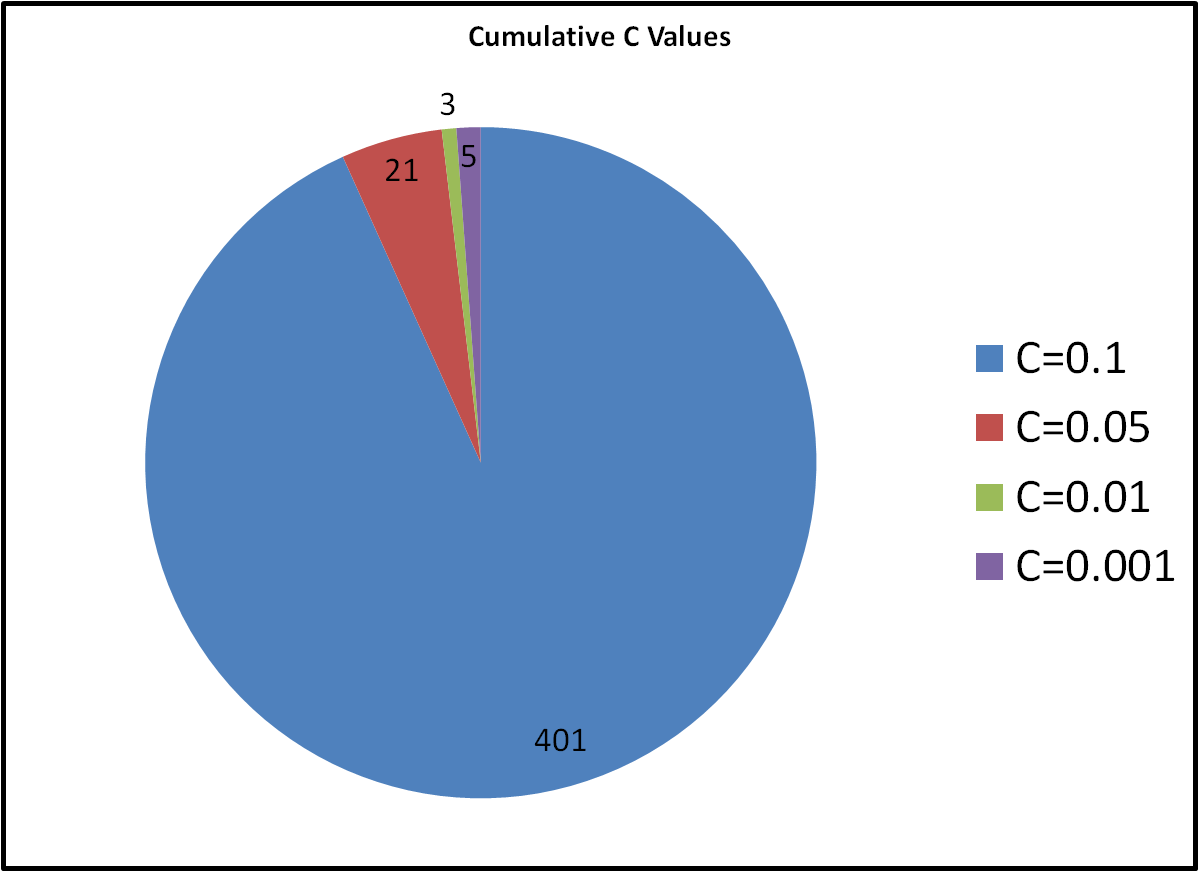
\includegraphics[width=\columnwidth]{c_values.png}
\caption{Hello}
\end{figure}

The results of tuning our support vector machines for each representative indicate that for most representatives a C value of 0.1 is the best. As can be seen in figure 1, the vast majority of optimized C values were 0.1 with small numbers of representatives' optimized C values being 0.05, 0.01, and 0.001.

The average accuracy of the optimized support vector machines on each representative's test set was 84.60\%, while the baseline model had an average accuracy of 80.80\% on those same test sets. Thus the optimized support vector machine had an average accuracy 3.80\% higher than that of the baseline model.

\begin{figure}
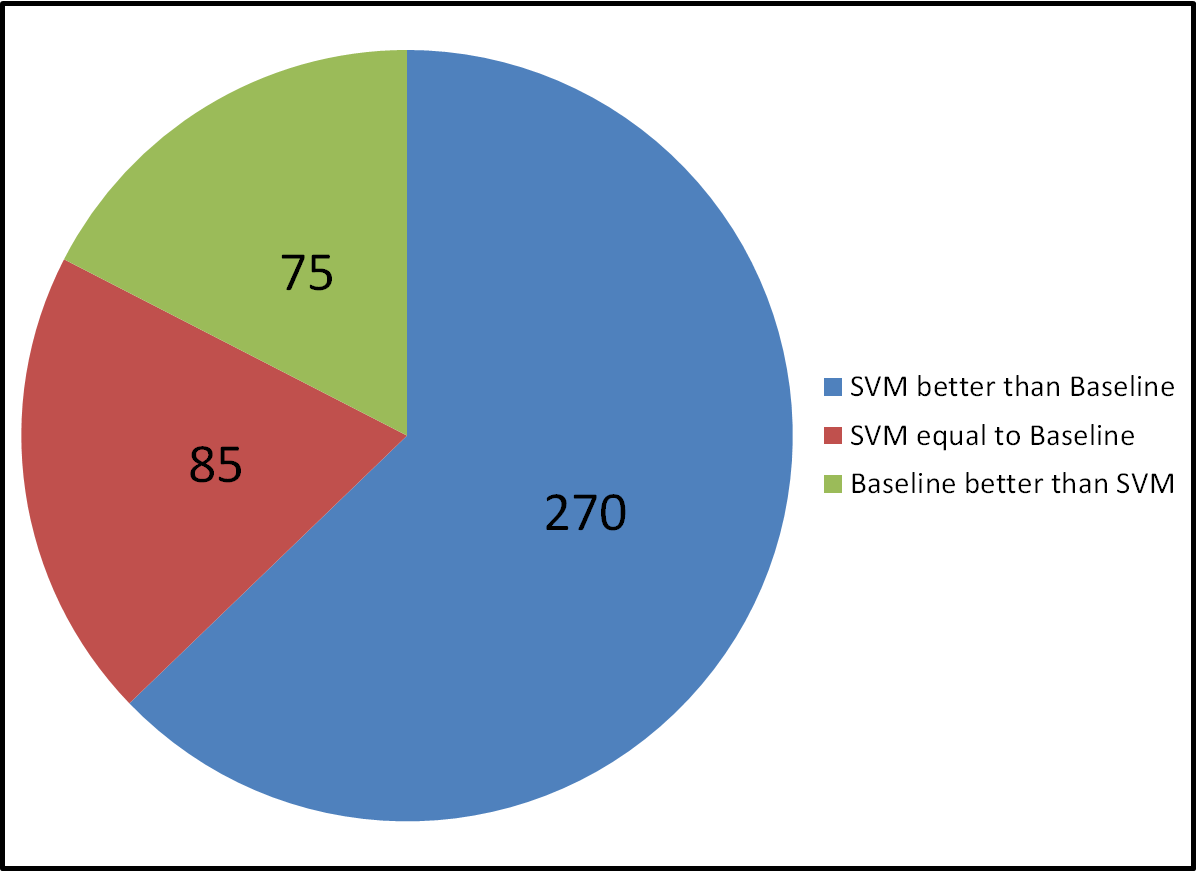
\includegraphics[width=\columnwidth]{pie_chart_1.png}
\caption{A pie chart comparing for how many representatives the support vector machine performs better than the baseline, how many each model performs approximately the same and for how many the baseline performs better}
\end{figure}

For 355 of the 430 representatives the support vector machine did as well as or better than the baseline. Of those 355 representatives, only eighty five had approximately equal results between the optimized support vector machine and the baseline hypothesis (Figure 2).

\begin{figure*}[t]
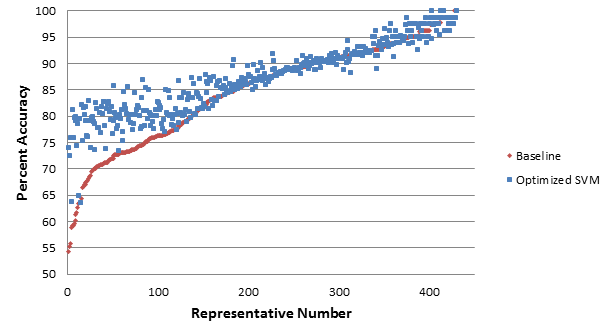
\includegraphics[width=\linewidth]{accuracy_comparison2.png}
\caption{A comparison of the baseline accuracy and optimized SVM accuracy sorted by representative such that baseline accuracy is increasing as representative number increases.}
\end{figure*}

As can be seen in Figure 3, the support vector machine's performance was particularly good in comparison to the baseline for representatives where the baseline had relatively poor test accuracy. For representatives on which the baseline test accuracy was higher the optimized support vector machines fell more into line with the baseline, typically doing better than it.

\begin{figure}
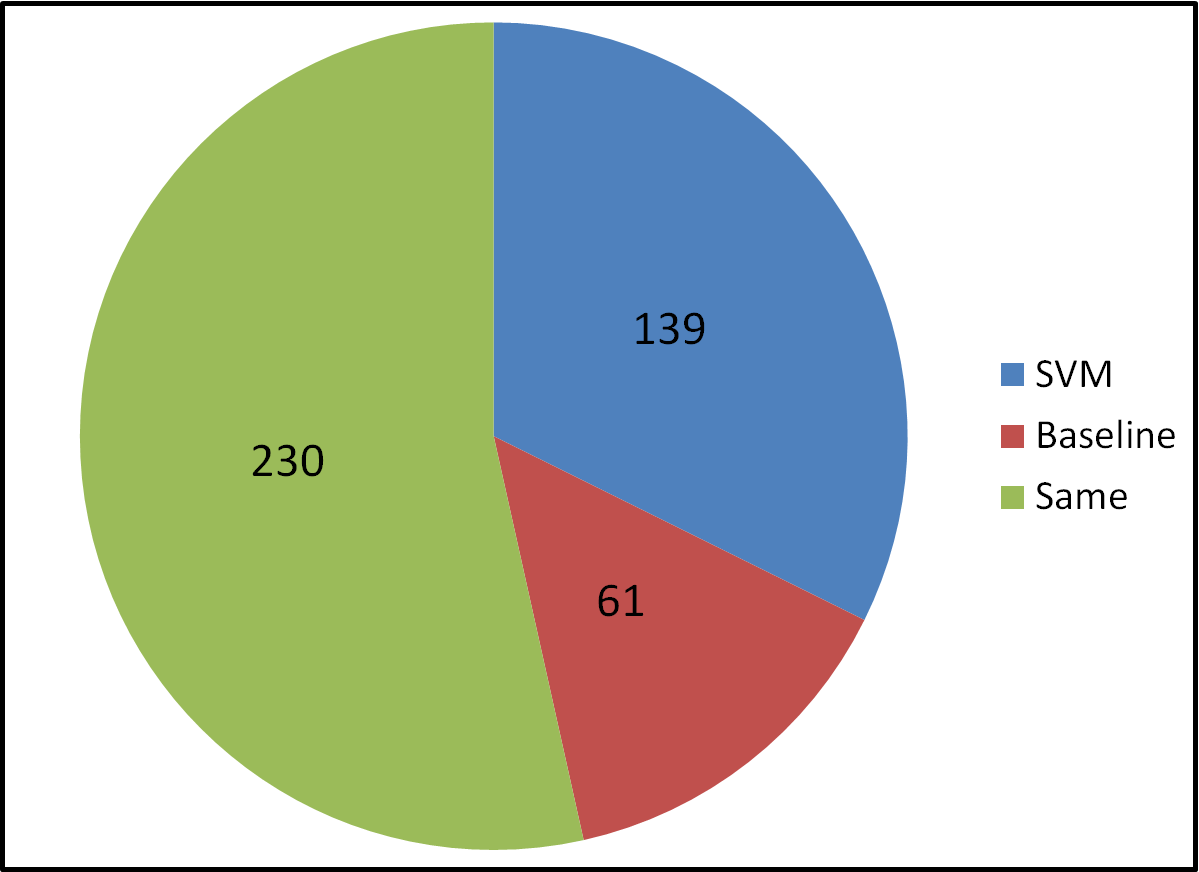
\includegraphics[width=\columnwidth]{mcnemar_results.png}
\caption{A pie chart showing the cumulative results of McNemar's Tests on each representative. "SVM" indicates the null hypothesis was rejected and the SVM performed better, vice versa for "Baseline" and "Same" indicates the null hypothesis could not be reject.}
\end{figure}

The results of our statistical analysis of the baseline hypothesis and the optimized support vector machines  can be seen in Figure 4. The results are similarly encouraging to the observational results detailed above. Cumulatively, for 139 representatives we can reject the null hypothesis of the McNemar's Test with 95\% confidence and say that the optimized support vector machine is a better hypothesis as it performed better in these 139 cases. For 61 representatives the opposite was true and the null hypothesis was rejected in favor of the baseline model. Thus for more than twice as many representatives the optimized support vector machines are better with 95\% confidence. This indicates that overall the optimized support vector machine model was a better hypothesis than the baseline model.

\begin{figure}
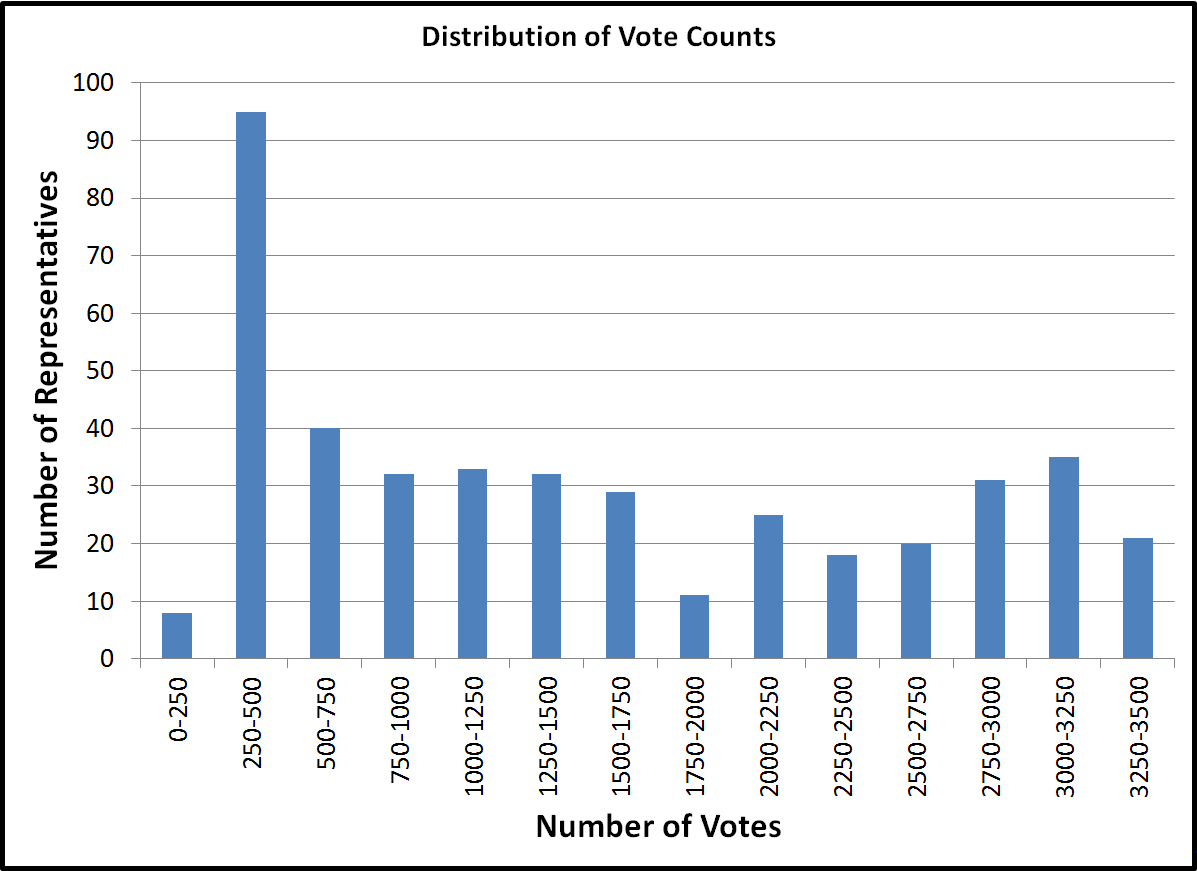
\includegraphics[width=\columnwidth]{data_distribution.png}
\caption{Histogram showing how many representatives have the number of votes within each bin.}
\end{figure}

We further examined our results to see how data sparseness could be affecting our results. As can be seen in Figure 5, for nearly a quarter of representatives have fewer than 500 votes each, giving us little data with which to work. Thus we were concerned that the amount of data we had for each representative may be affecting the performance of the baseline model and the support vector machine model.

\begin{figure*}[t]
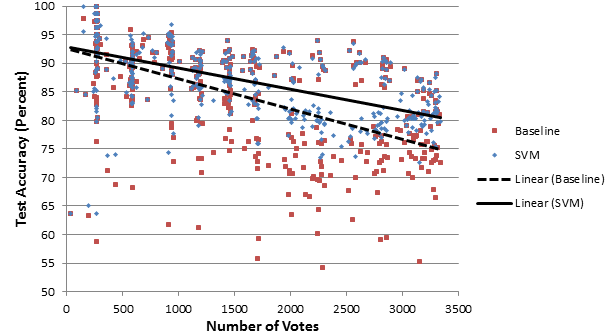
\includegraphics[width=\linewidth]{size_accuracy2.png}
\caption{Comparison of test accuracies between baseline and optimized support vector machine, representatives sorted by number of votes. Linear trendlines included to show trends.}
\end{figure*}

In Figure 6, the performance of the baseline and the optimized support vector machines on the test sets can be seen, with representatives sorted by the number of votes we had for each, from smallest to largest. As can be seen by the trendlines, both models test accuracy decline slightly as the number of votes increases; however, the baseline accuracy decreases more than the optimized support vector machine. Further it can be seen that test accuracies appear to vary less as the number of votes increase.

\begin{table}
\centering
\begin{tabular}{|c|c|} \hline
Percent of House & Prediction \\ \hline
0.565 & Pass \\ \hline
0.588 & Pass\\ \hline
0.586 & Pass\\ \hline
0.574 & Pass\\ \hline
0.804 & Pass\\ \hline
0.591 & Pass\\ \hline
\end{tabular}
\caption{Table showing the ratio (percent) of the weighted sum of predicted "yea" votes to the weighted sum of predicted "nay" votes as well as whether passage was predicted.}
\end{table}

We did no thorough examination of predicting passage of bills. Due to the sparseness of our data (Figure 5) we used every bill that we could for training, validation and testing. That left us with six bills that had been voted on for passage in the month after we originally pulled our data. We then used our model for predicting bill passage on each of these six bills. As can be seen in Table 1, above, we correctly predicted that each bill passed. 

\section{Discussion}

\section{Related Work}

The only work similar to ours as described here was conducted by Princeton researchers Garrish and Blei and described in their paper \textit{Predicting Legislative Roll Calls from Text}. Their work focuses upon the text of bills for which there were roll call votes, using only text to predict votes and their work spanned both the Senate and the House of Representatives (Gerrish \& Blei, 2011). They developed models for votes which extended the ideal point model from political science, which places a representative in space, this point being their ideal point, and bills in the same space (Gerrish \& Blei, 2011). The vote of the congressperson is a function of his or her ideal point and the location of the bill in the space. From this initial model they developed three models: The Bayesian ideal point model, ideal points with text regression and an ideal point topic model (Gerrish \& Blei, 2011). 

The Bayesian model is a generative model for predicting votes. It uses the ideal point of the congressperson and the bill's ideal point, biased by a term which accounts for how much plitical division a bill has and applies a logistic regression with random effects to the result (Gerrish \& Blei, 2011). 

The text regression model takes the ideal point model and fits a training set to it and then applies a regression model to it (Gerrish \& Blei, 2011).

The ideal point topic model takes text of bills to come up with the topic of a bill and relates it to sentiment on the bill (Gerrish \& Blei, 2011).

Our problem is far different. We do not limit our bills to roll call votes and instead of focusing on both the Senate and the House we look only at the House. Further we do more than predict individual votes, but also take our individual predicts and use them to predict bill passage. Gerrish and Blei used the text of bills to create various extended ideal point models to predict how a congressperson will vote. We do not use the ideal point model, or any of the machine learning techniques applied by Gerrish and Blei. Instead we use a support vector machine and metadata about bills, rather than bill text. Our problem is more general in its scope and has further applications to the general public and industry, as predicting bill passage could prove to be useful for  corporations and citizens. Further our approach is simpler, applying the commonly used support vector machines to small, computationally inexpensive feature vectors easily pulled from bill metadata.
 
\section{Future Work}

\section{Conclusion}

\section*{Acknowledgments}

We would like to thank Igor Labutov and Thorsten Joachims for their advice and guidance on this work. We would also like to thank the entire CS4780 course staff, Cornell University and Govtrack. 

\pagebreak

\section*{References}

Gerrish, S. M., \& Blei, D. M. (2011). Predicting legislative roll calls from text. International Conference on Machine Learning

\end{document}